\chapter{State of the art}
\label{ch:state_of_the_art}
In the following chapter we are first going to examine level design from an historical and industry perspective, with a particular focus on First-Person Shooter (FPS) games and academic research on the topic of level design for FPS games.

Then we are going to look at how balancing is defined and what elements of multiplayer games make a game balanced. Specifically, we are also going to examine how maps influence the balance of FPS games.

We will also review the history of commercial games utilizing Procedural Content Generation (PCG) and provide a taxonomy of the approaches used, including an examination of Search-Based PCG. Furthermore, we will analyze the state of the art in academic research on PCG for maps in FPS games.

Finally, we will look into Quality Diversity methods, specifically at MAP-Elites, and present how it has been used in the literature to generate videogame content.

\section{Level design in First-Person Shooter games}
\label{sec:level_design}
In the field of game design and development, level design can be defined as the discipline of crafting video game levels, places and missions to achieve gameplay that is both fun and balanced, leveraging genre and game-specific mechanics.

In the early days of video game development, game programmers also doubled as level designers, but as the industry grew bigger the importance of a dedicated level designer role became apparent. Level design is arguably the biggest factor in ensuring that the player is always engaged and that the gameplay mechanics are fully utilized. Despite this, level design, as a discipline, doesn't yet have clearly defined processes and terminology and instead relies on the talent and experience of talented individuals.

A number of books have been written on the topic, most of which discuss common practices and describe the tools used by level designers, but don't detail how level design creates gameplay. As an example, in his book \textit{Level Design for Games: Creating Compelling Game Experiences}, \Citeauthor{co_level_2006} explains the process of designing a level for an FPS game in practical detail, starting from a brainstorming phase, through building the level in Unreal Engine\footnote{Game engine developed by Epic Games.}, and to finally testing and improving the level \cite{co_level_2006}, but does not delve in how this process creates gameplay. \cite{hullett_design_2010}

Shorter academic works have focused on certain aspects of level design which are independent of genre: some have focused on gameplay idioms such as correctly pacing the level, creating tension and creating a suitable level of challenge, while others focused on spatial characteristics of the playing environment, such as the spatial configurations or how the player navigates the level. \cite{hullett_design_2010}

In First-Person Shooters (FPS)\footnote{First-Person Shooters are a genre of video games that are played from the perspective of the player character and that revolve around gun-fighting, such as \textit{Wolfenstein 3D} (id Software, 1992), \textit{Doom} (id Software, 1993) and \textit{Quake} (id Software, 1996).} level design takes the form of designing the level or map that the player is placed in, minding the placement of objects, covers and enemies. There exist many kinds of FPS games, each with different gameplay mechanics (e.g. \textit{Titanfall}\footnote{Respawn Entertainment, 2014}, which allows the player to run on walls) and level design principles. 

The most important distinction that can be drawn is between singleplayer and multiplayer FPS games. Singleplayer games usually see the player traversing a level in linear fashion, completing objectives defined by the game designer, such as solving puzzles or defeating enemies, and optionally discovering secrets or uncovering a story, such as in \textit{Half-Life}\footnote{Valve Corporation, 1998}. In multiplayer games like \textit{Call of Duty}\footnote{Infinity Ward, 2003} players compete to achieve a goal before their opponent (e.g. capture the flag, kill the enemy team) and the levels are designed to facilitate and balance this competition. Other multiplayer games may instead require players to cooperate to reach a common goal, such as in \textit{Left 4 Dead}\footnote{Valve Corporation, 2008}, where players have to survive a zombie apocalypse together or in \textit{Portal 2}\footnote{Valve Software, 2011}, where players have to solve puzzles together.

The differences between these types of games are reflected in the level design principles that are used. While singleplayer and cooperative games may thrive from having maps that put the player in a position of disadvantage to increase challenge and tension, competitive multiplayer games require maps that are balanced and fair to all players. 

Given that FPS games usually also present multiple game modes that naturally require diverse level designs, academic research has either focused on a singular and more universal aspect (such as pace, challenge or tension), or has tried to analyze a specific game (or type of game) to examine a specific feature of its level design.


\Citeauthor*{guttler_spatial_2003} outlined the basic spatial principles of level design in multiplayer First-Person Shooters with special reference to \textit{Counter-Strike} \cite{guttler_spatial_2003}. They argue  that successful level design for multiplayer FPS is based on several factors, such as gameplay, theme, architecture and spatial structure, and that the level designer will greatly benefit from leveraging theoretical tools to develop maps, as such tools would make  eliciting specific gameplay during game sessions easier. By analyzing the gameplay of existing maps and their layouts they deduce the basic spatial principles of \textit{Counter-Strike}'s level design and elaborate on how to best apply them to create a successful map. 

\Citeauthor{larsen_level_2006} argues the usefulness of patterns in fields ranging from software development to film making, and proposes that they can be used to describe level design practices in the domain of FPS games. He specifically focuses on several competitive multiplayer FPS games (\textit{Unreal Tournament 2004}\footnote{Epic Games, 2004}, \textit{Day of Defeat: Source}\footnote{Valve Corporation, 2005} and \textit{Battlefield 1942}\footnote{DICE, 2002}) and extracts common design patterns by analyzing several levels in search of common ways of solving problematic elements. He defines the patterns of "multiple paths", "local fights", "collision points", "reference points", "defense areas" and "risk incentive". For each identified pattern, he provides a description, examples on how to use the pattern, consequences on gameplay, how it interacts with other patterns and commercial examples of its use. He concludes that recurring patterns should not streamline levels but instead be used as tools to design better levels. \cite{larsen_level_2006}

In a similar vein, \Citeauthor*{hullett_design_2010} adapt how patterns are characterized in the field of software engineering to the domain of single player FPS level design. They use this characterization to identify a set of design patterns commonly used in FPS level design, which can be used as a language for describing design practices in the domain of FPS games. Patterns are divided into "patterns for positional advantage" (sniper locations, gallery, choke point), "patterns for large scale combat" (arena, stronghold), "patterns for alternate gameplay" (turret, vehicle selection) and "pattern for alternate routes" (split-level, hidden area, flanking route). For each, they provide a description, how it can be modified, the gameplay it creates, how it interacts with other patterns and commercial examples of its use. 
They argue that patterns can help designers generate new ideas by combining them, and can also help solve design problems by providing guidance on what to add or remove to achieve a gameplay goal, since patterns offer a clear cause-effect explanation. They also argue that these patterns can be generalized and reasonably applied to multiplayer games in some situations. \cite{hullett_design_2010}

\section{Balance in competitive multiplayer video games}
\label{sec:balance}
A concept that is closely related to level design is \textit{game balance}. Giving a general definition for "game balance" is a harder task than it might seem, as \citeauthor{becker_what_2020} note in their semantic analysis based on other publications on the theme of balancing games of various kinds. They conclude that further research would be needed to reach a commonly agreeable definition, given that the authors they analyzed did not have a common central goal, with some focusing on the end goal of "fun", other on "challenge" and others on "flow". \cite{becker_what_2020}

For multiplayer games specifically, \citeauthor{sirlin_balancing_2014} states that a game is balanced if the player can choose between a sufficiently large array of options which are viable, meaning that they are different, meaningful and not dominated by other options. These choices can be made before the game starts (fairness) or during the game itself (viable options). \cite{sirlin_balancing_2014}

When players can choose between different sets of options before starting the game we talk about \textit{asymmetric games} (e.g. most FPS games where you can select your weapon, or fighting games with multiple playable characters), while in \textit{symmetric games} players start the game with an identical and static set of options (e.g. games like Tetris\footnote{Aleksej Pažitnov, Vadim Gerasimov, Dmitrij Pavlovskij, 1984}, where players are fed the same pieces during the competition) \cite{sirlin_balancing_2014}. The former are naturally easy to balance, but often games introduce options to stand out and make the game more replayable, deep and fun; a fighting game with only a single character would surely be balanced, but also boring. 

A concept that \citeauthor{sirlin_balancing_2014} highlights is that of "dominant strategies". For a competitive game to be balanced a player should be able to choose at any time between many viable options, but if one of those is too strong it would both make other options meaningless and reduce the strategic value of the game. To allow for a balanced game with deep strategy it can be beneficial to consider the concept of "Yomi"\footnote{A Japanese word that can be translated to "Reading". In this context, it is meant as "reading the mind of your opponent".}, which refers to the fact that if a player were to read the opponent's mind, he should then be able to counter the opponent's strategy. A dominant strategy is one so strong that counters may not exist. \cite{sirlin_balancing_2014}

When strictly considering asymmetric games, authors agree that balancing should not be the sole goal \cite{sirlin_balancing_2014} \cite{portwnow_perfect_2012} \cite{brown_how_2019}. These games are designed to allow players to employ various strategies and tactics, so while no one strategy should be strictly better than others, if all strategies were instead perfectly balanced the game may provide un-fun options that feel very similar to each other \cite{sakurai_amplify_2024}. The player's perception of balance is sometimes more important than balance itself to provide players with a fun experience \cite{brown_how_2019}, which makes correctly balancing the game a difficult task that can't be fully understood by merely examining the win rates\footnote{The number of times a character/strategy wins over a certain number of matches.}. Developers must also take into account the "pick rate" of certain characters or strategies, the skill level of players, the skill required to employ a given strategy and the \textit{meta-game}\footnote{Term that refers to the strategies that are popular at a given time among the player-base, due to their strength and/or their ease of use.} to correctly balance a game. \cite{brown_how_2019} 

Many competitive games, such as Real Time Strategy (RTS) games, Multiplayer Online Battle Arena (MOBA) and FPS games, are played on certain maps whose design could greatly influence the outcome of the match. Because different players or teams may have distinct play-styles, some may gain an advantage in playing certain maps compared to others, and creating a map fair to every existing style of play may be unfeasible. For this very reason, during official competitions, popular competitive games like \textit{Counter Strike: Global Offensive}\footnote{Valve Corporation, 2012} or \textit{Super Smash Bros. Ultimate}\footnote{Bandai Namco Games, Sora Ltd., 2018} allow competitors to take turns in "banning"\footnote{In this context, a "ban" (often also called "strike") means disallowing the opponent from choosing a specific map for the next match.} a map, so that the final chosen map is one that both players are comfortable playing on.

Moreover, what makes a multiplayer map balanced highly depends on the specific game mechanics and the game mode that is being played. In the "capture the flag" game mode\footnote{Popular game mode where two teams face off, and each one has to infiltrate the opposing base to steal a flag and bring it back to their own base.} two teams have to achieve the same objective, so a balanced map can be achieved with a symmetrical layout, as in Team Fortress 2\footnote{Valve Corporation, 2007} (Figure \cref{fig:ctf_tf2}). \textit{Counter-Strike} instead has a "Bomb Defusal" game mode\footnote{Game mode where a team, the "Terrorists", must place and detonate a bomb while the other team, the "Counter-Terrorists", has to defend designated locations.} where a balanced map will probably have an asymmetrical layout, where, for example, the defending will spawn closer to the areas they will have to defend in order to organize themselves, while the attacking team will have multiple attacking routes to the sites (Figure \cref{fig:dust2}).

\begin{figure}[hbt!]
    \centering
    \subfloat["Thunder mountain", a Capture the Flag map in \textit{Team Fortress 2}.\label{fig:ctf_tf2}]{
        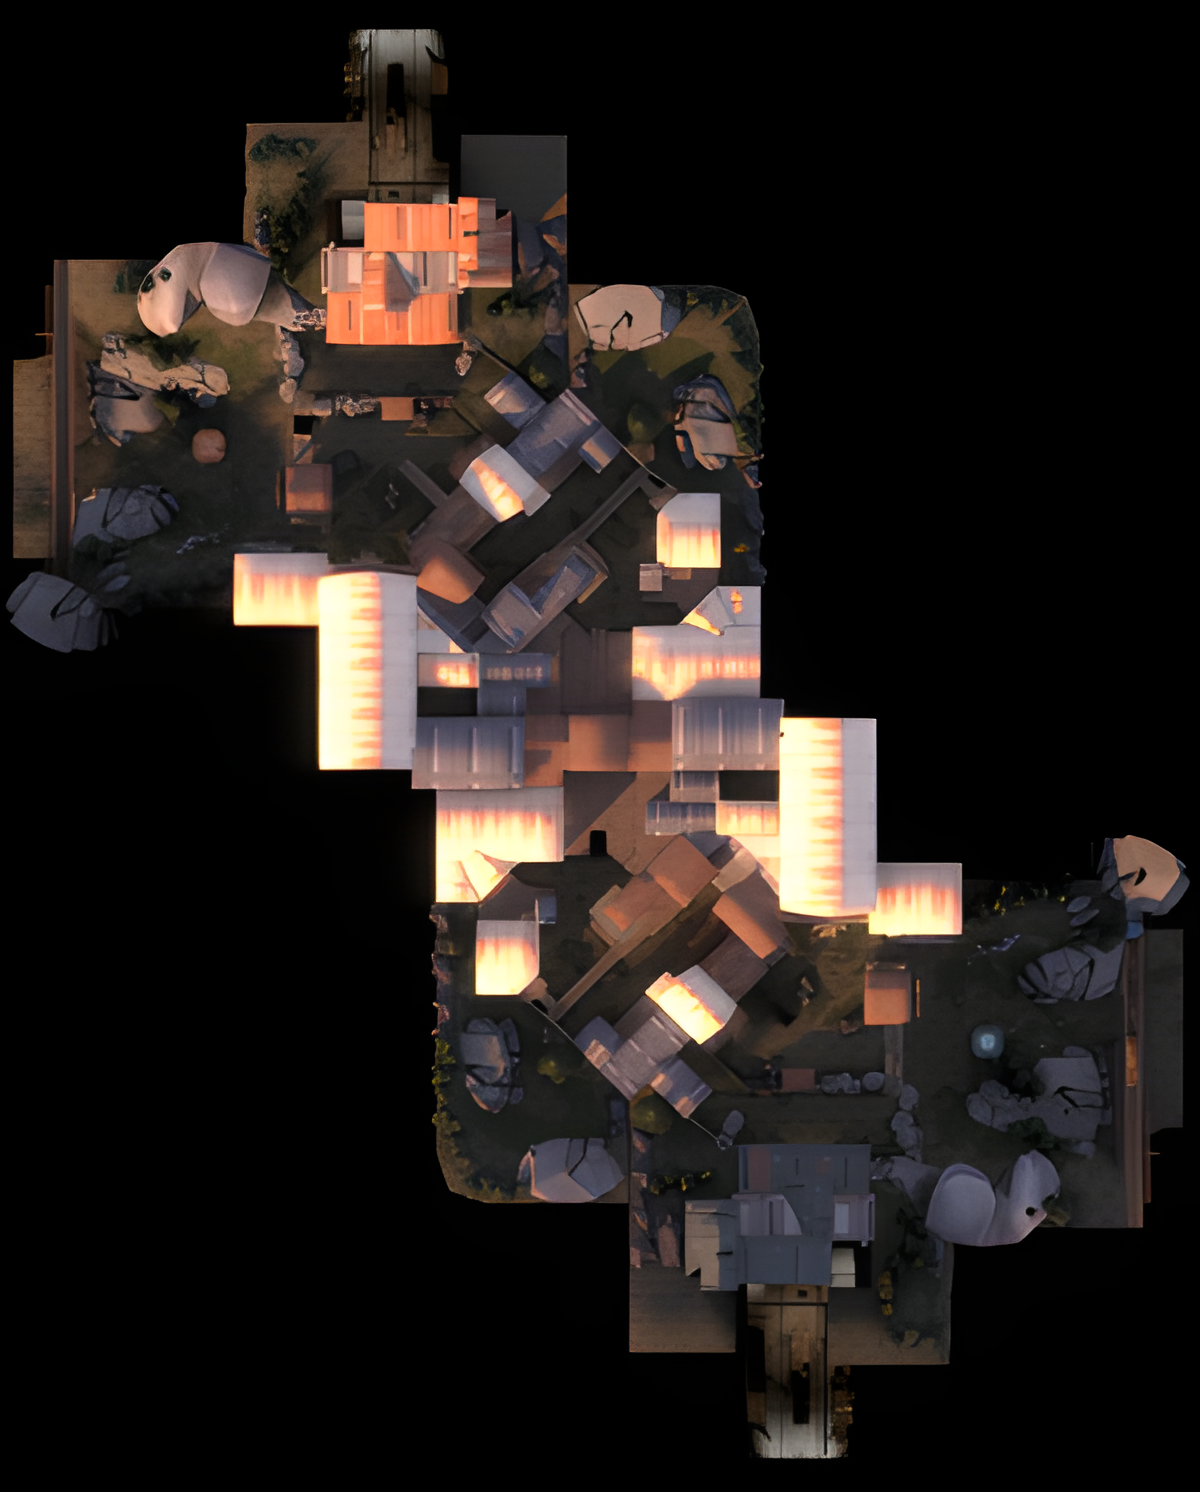
\includegraphics[height=0.4\textwidth]{Images/Thunder_Mountain_(Capture_the_Flag).png}
    }
    \quad
    \subfloat["Dust II", a Bomb Defusal map in \textit{Counter-Strike}.\label{fig:dust2}]{
        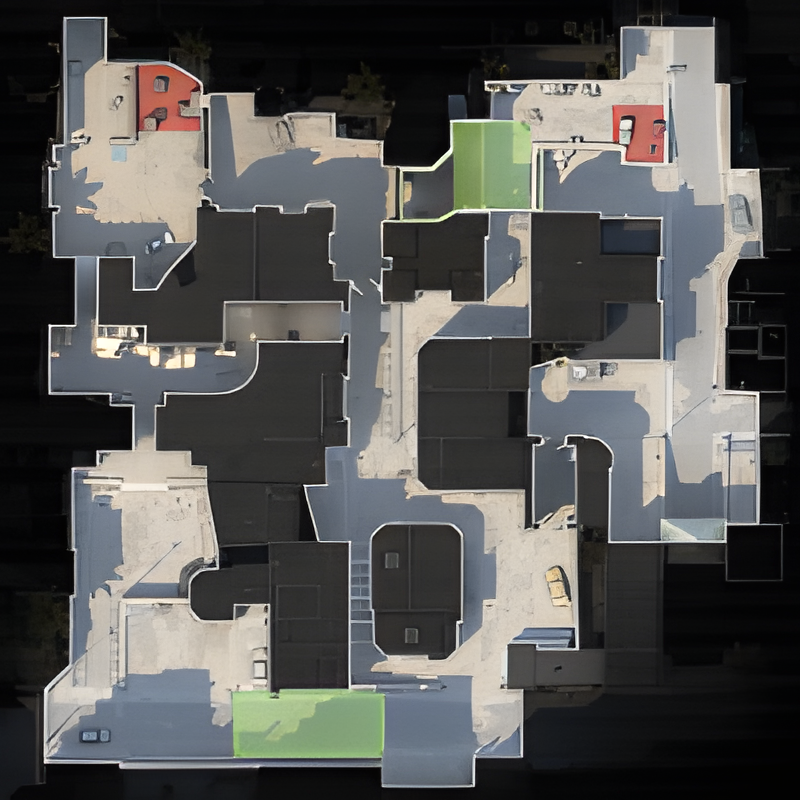
\includegraphics[height=0.4\textwidth]{Images/Dust_II.png}
    }
    \caption[Map comparison]{Comparison of a symmetrical "Capture the Flag" map with an asymmetrical "Bomb Defusal" map.}
    \label{fig:maps_compare}
\end{figure}

Even considering a single game mode, such as "deathmatch"\footnote{Game mode where players, optionally divided in teams, compete in order to score the most kills.}, the number of players in a team drastically changes the tactics that are employed, and the level design should account for that. Games that focus on 1v1 combat (e.g. \textit{Unreal Tournament 2004}) will usually have fast movement and dynamic gameplay that rewards reflexes and mechanical skills, so maps will have multiple floors with various escape routes but will be relatively small and with numerous collision points that make it hard to hide. Instead, games that are mainly played in teams (e.g. \textit{Battlefield 1942}) will have bigger maps with few collision points allowing teams to strategically position themselves to gain control of these sections.

The observations made in this section about balancing maps in competitive FPS games may seem like "common sense", however \citeauthor{johnston_common_2003}, author of the popular "Dust II" map in figure \cref{fig:dust2}, argues that the best asset a level designer has is their common sense, and uses practical examples to guide readers on how to create balanced and fun maps \cite{johnston_common_2003}.

Finally, we note that there is a lack of academic research on the topic of balancing maps in competitive FPS games, which leads to a lack of a clear methodology to follow when designing and balancing a map, having instead to rely on "common sense", trial and error, observation and experience.  

\section{Procedural content generation in games}
\label{sec:procedural_content_generation}
We refer to \textit{Procedural Content Generation} (PCG) as the process of creating game content algorithmically, rather than manually. This can be used to create levels, characters, items, quests, dialogues, and more. 

PCG has been used in games since the early days of the industry, with games like \textit{Rogue}\footnote{A.I. Design, 1980} using procedural generation to create levels, items, and enemies. The technique has helped developers create games that use less storage space and have more replayability. To this day, many successful games that span many genres employ PCG to create content, such as \textit{Minecraft}\footnote{Mojang, 2011}, \textit{No Man's Sky}\footnote{Hello Games, 2016}, the \textit{Mystery Dungeon}\footnote{Chunsoft, 1993} series or \textit{Hades}\footnote{Supergiant Games, 2020}.

\begin{figure}[hbt!]
    \centering
    \subfloat[\textit{Minecraft}\label{fig:Minecraft}]{
        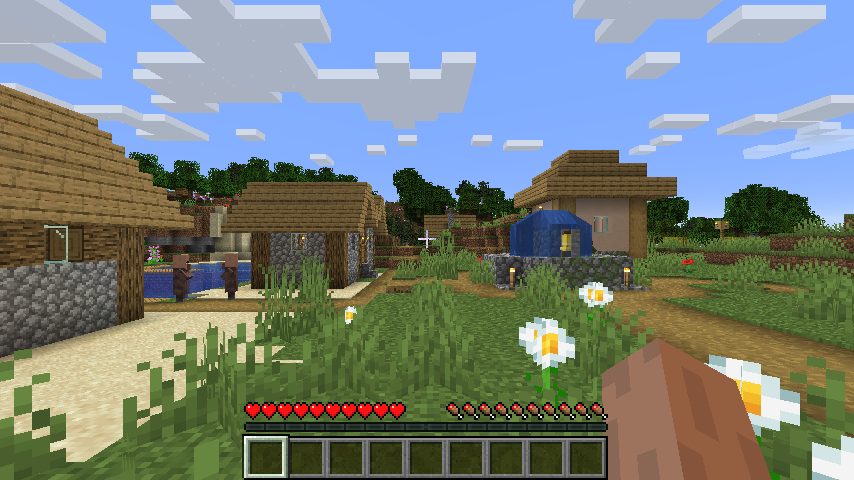
\includegraphics[height=0.2\textwidth]{Images/Minecraft.png}
    }
    %\quad
    %\subfloat[\textit{No Man's Sky}\label{fig:nms}]{
    %    \includegraphics[height=0.2\textwidth]{Images/nms.png}
    %}
    \subfloat[\textit{Pokémon Mystery Dungeon: Explorers of Sky}\label{fig:md}]{
        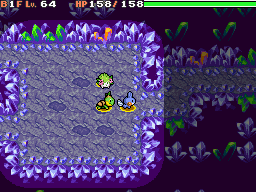
\includegraphics[height=0.2\textwidth]{Images/MD.png}
    }
    \subfloat[\textit{Hades}\label{fig:hades}]{
        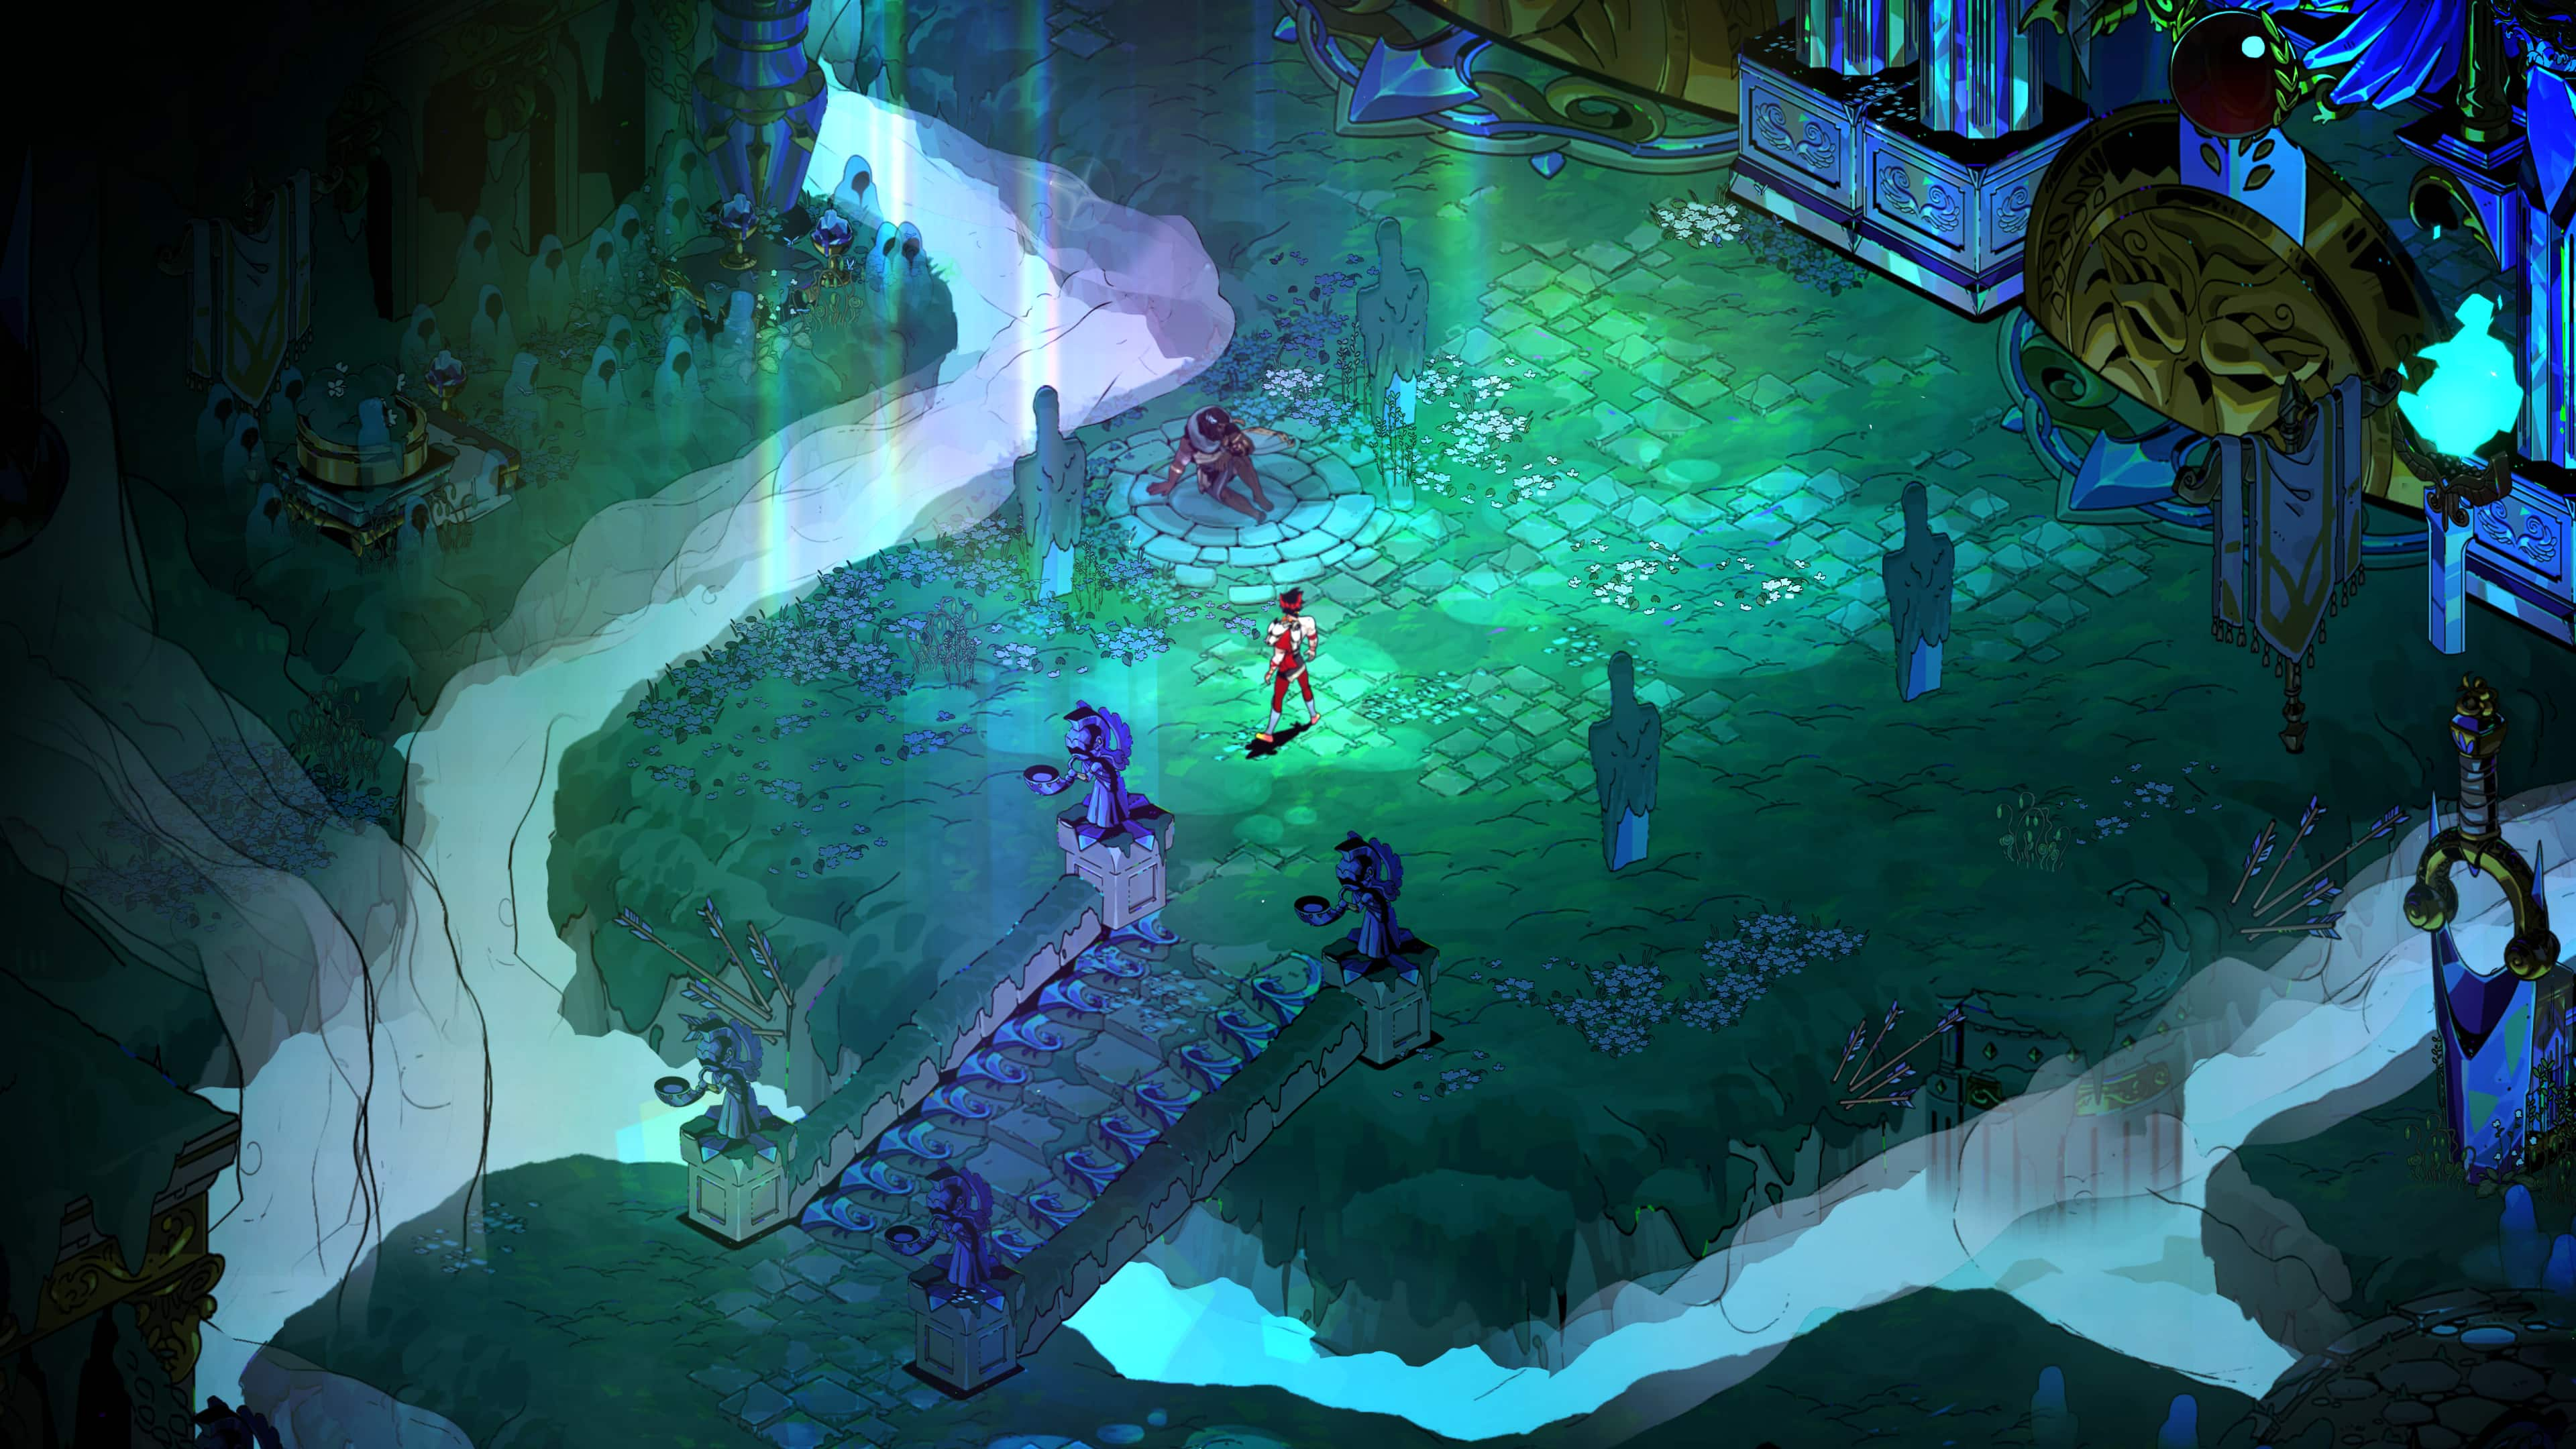
\includegraphics[height=0.2\textwidth]{Images/Hades.jpg}
    }
    \caption[PCG Games]{Examples of diverse games that use PCG to create content.}
    \label{fig:pcg_games}
\end{figure}


In the domain of FPS games PCG has mostly been used for single player games or multiplayer collaborative games. The already cited \textit{No Man's Sky} uses PCG to create an entire universe of planets, each with its own flora, fauna, and resources. \textit{Borderlands}\footnote{Gearbox Software, 2009} uses PCG to create weapons with different stats and abilities, while \textit{Deep Rock Galactic}\footnote{Ghost Ship Games, 2018} creates levels that are different each time a mission is played. However, there are no critically acclaimed multiplayer competitive games that use PCG to create levels yet.

\Citeauthor*{togelius_search-based_2010} offer a taxonomy of PCG approaches used in games by drawing some distinctions between them. First, they note the difference between \textit{online} approaches, which generate content as the game is played, and \textit{offline} approaches, which generate content during the development phase. Then they distinguish between \textit{necessary} and \textit{optional}, depending on whether the content generated is mandatory to finish the game. Another distinction is between \textit{random seeds} and \textit{parameter vectors}; the former simply takes a single seed to generate content, while the latter uses more parameters. The amount of randomness can classify an approach as either \textit{stochastic} or \textit{deterministic} and, finally, they distinguish \textit{constructive} approaches, where the content is generated once, ensuring that it is correct and good during the creation process itself, and \textit{generate-and-test}, where the content is first generated and then tested, and the algorithm is possibly repeated to produce better content. \cite{togelius_search-based_2010}

\subsection{Search based procedural content generation}
\label{subsec:search_based_pcg}
Referring to the taxonomy of PCG approaches just defined, \textit{Search Based Procedural Content Generation} (SB-PCG) is a particular case of \textit{generate-and-test} PCG, where the content is first generated, then the candidate is tested and evaluated with a \textit{fitness function}, and the generation of a new candidate depends on the result of this evaluation. \cite{togelius_search-based_2010}

\begin{figure}[hbt!]
    \centering
    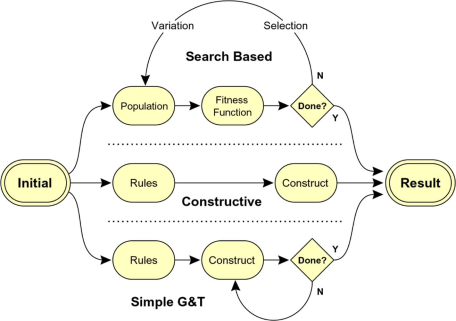
\includegraphics[width=0.6\textwidth]{Images/Togelius.png}
    \caption{Comparison of SB-PCG with constructive and generate-and-test approaches.}
    \label{fig:pcg}
\end{figure}

Among search-based PCG methods, \textit{Evolutionary Algorithms} (EA) make up most of them. \cite{togelius_search-based_2010}

An EA is a population-based optimization algorithm that mimics the process of natural selection, borrowing some concepts from biology and genetics. An algorithm of this family proceeds in cycles, often called epochs or generations. The first epoch starts with generating an initial population of candidates (or individuals), then each candidate in the population is evaluated with a fitness function and the best are selected to reproduce using crossover or mutation, creating new candidates that will replace the worst scoring individuals, giving rise to a new population, which will be the starting point of the next epoch. This process is repeated for a number of generations, and the algorithm ends when a stopping criterion is met, like a reaching certain number of generations or finding an individual with a particularly high fitness. \cite{lones_sean_2011}

An important concept that is loosely taken from biology is that of \textit{genotype} and \textit{phenotype}. EAs usually cannot work directly on the final content they are trying to generate, such as maps or 3D models, and they instead work on a low-level representation that may employ different parameters and data structures to describe the candidate's content. This representation should also allow the algorithm to apply crossover and mutation in a computationally fast and meaningful way. Each genotype is then mapped to a phenotype, which is the final content, that can be evaluated by the fitness function. \cite{togelius_search-based_2010}

Choosing the right genotype and genotype-to-phenotype mapping is crucial to the success of the algorithm, and many factors must be taken into account. 

Firstly, it is important to choose a genotype representation with the right number of parameters; an encoding having few parameters may be unable to represent the content or introduce bias in the search space, while having too many parameters may make the search space too large to be effectively explored by the algorithm\footnote{This phenomenon is called the \textit{curse of dimensionality}, referencing how having too many dimensions in a search is often detrimental to the search itself.}.
A good genotype representation will also sport good locality, meaning that a small change in the genotype should result on average in small changes in the phenotype.
A genotype encoding should also be able to represent all interesting solutions, which could be hard to achieve while avoiding the use of too many parameters. \cite{togelius_search-based_2010}

A genotype that is one to one with the phenotype (which is classified as a \textit{direct encoding}) will often lead to a search space that is too large to be effectively searched by most EAs, as we would need too many parameters to describe all the details of the phenotype. Using instead a single parameter, such as a random seed, to generate the phenotype (which is classified as \textit{indirect encoding}, as we need a complex computation to obtain the phenotype from the parameters) may lead to very poor locality, since, by definition, a good random number generator will show no correlation between the numbers generated by neighboring seed values. Choosing the correct balance between these two extremes is crucial to the success of the algorithm and requires knowledge of the domain. \cite{togelius_search-based_2010}

Another crucial factor of an EA is the fitness function. First, it must be defined what is the objective of the search, then the fitness function must be formalized. The process of defining the fitness function is complex as it requires domain-specific knowledge and depends on the objective of the search; to define how hard a level is to play we can leverage objective data, such as how many times a player dies or where he died, but formalizing abstract concepts, such as how much fun a level is to play, will surely rely on conflicting assumptions and subjective opinions, which could make our evaluation imprecise and unreliable. \cite{togelius_search-based_2010}

We can classify fitness functions in 3 categories \cite{togelius_search-based_2010}:
\begin{itemize}
    \item \textit{Direct fitness functions}, where features are extracted directly from the generated content and used to evaluate it. These functions are usually fast to compute, but many features may be hard, if not impossible, to define directly.
    \item \textit{Simulation-based fitness functions}, where an agent plays the game content generated and simulation data is recorded, which is then used to evaluate the candidate. This method is slower to compute as simulations take time to run, but it allows for a vaster range of features to be evaluated. 
    \item \textit{Interactive fitness functions}, where the candidate is evaluated by a human player and implicit (e.g. game data) or explicit (e.g. questionnaires) feedback is collected. This method avoids the inherent bias issues that arise when using bots by using human players instead, at the cost of both needing a playerbase and evolution taking longer, since the game cannot be sped up.  
\end{itemize}


\subsection{Procedural map generation in competitive FPS games}
\label{subsec:pcg_fps}
While no acclaimed commercial game uses PCG to create maps for competitive multiplayer games, some academic research has been done on the topic.

\citeauthor{cardamone_evolving_2011} have started research in this field by using search-based techniques to generate playable FPS maps for the "deathmatch" game mode of \textit{Cube 2: Sauerbraten}\footnote{Lee Salzman, Wouter van Oortmerssen, Mike Dysart, Robert Pointon, 2004}. In their work they defined four different genotypes (\textit{All-White}, \textit{All-Black}, \textit{Grid} and \textit{Random-Digger}, in figure \cref{fig:map_genomes}), and mapped each to a phenotype that can be used to generate a map for Cube 2. The candidate maps are evaluated using a simulation-based fitness function; each map is played for 10 minutes by 4 bots and the fitness is based on the \textit{average fighting time}, that is defined as the amount time passed from the moment in which the player starts to fight an opponent to the moment in which the player is killed. They argue that interesting maps will have features, such as escape routes and well-placed resources, that allow for long fights to happen. \cite{cardamone_evolving_2011}

\begin{figure}[hbt!]
    \centering
    \subfloat[\textit{All-White}\label{fig:allwhite}]{
        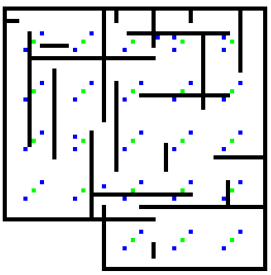
\includegraphics[height=0.2\textwidth]{Images/aw.png}
    }
    \quad
    \subfloat[\textit{All-Black}\label{fig:allblack}]{
        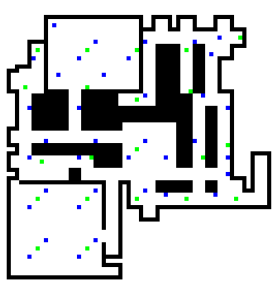
\includegraphics[height=0.2\textwidth]{Images/ab.png}
    }
    \subfloat[\textit{Grid}\label{fig:grid}]{
        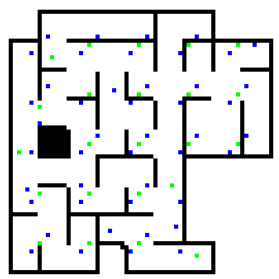
\includegraphics[height=0.2\textwidth]{Images/Grid.png}
    }
    \subfloat[\textit{Random-Digger}\label{fig:randomdigger}]{
        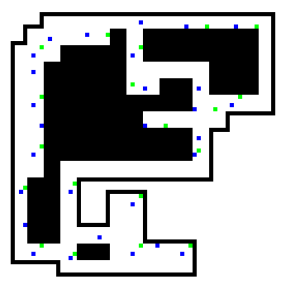
\includegraphics[height=0.2\textwidth]{Images/rd.png}
    }
    \caption[\citeauthor{cardamone_evolving_2011} example maps]{Different maps evolved by \citeauthor{cardamone_evolving_2011} with different genotypes.}
    \label{fig:map_genomes}
\end{figure}


Their work both proved the possibility of using an EA to evolve FPS maps and highlighted how different representations lead to maps with different topological characteristics, noting how some genomes were more suited to their objective.

\Citeauthor{lanzi_evolving_2014} have instead focused on evolving maps for \textit{Cube 2: Sauerbraten} that are balanced for a 1-vs-1 "deathmatch" game mode, simulated by agents which have differing skill levels and play styles. Leveraging the \textit{All-Black} genotype defined by \Citeauthor{cardamone_evolving_2011}, they employed a simulation-based fitness function based on \textit{entropy}, a measure of the match's balance based on the number of kills of each player. \cite{lanzi_evolving_2014}

\Citeauthor{olsted_interactive_2015} moved to evolving maps for the game \textit{FPSEvolver} focusing on the "Bomb Defusal" game mode, similar to that of \textit{Counter-Strike}. They argue that this game mode encourages more tactical planning and teamwork and that maps obtained by \Citeauthor{cardamone_evolving_2011} were unsuitable for this purpose, as they contained few dedicated arenas and many dead-ends. To obtain engaging maps they define a set of guidelines (named "\textit{the good engagement}") and a new genotype that by design creates layouts that adhere to these concepts, avoiding dead ends and ensuring arenas. They then employed \textit{iterative evolutionary computation} to evolve maps, requiring real users to play the maps. Users are then asked to leave binary feedback that is used to guide the evolution. \cite{olsted_interactive_2015}

\Citeauthor{loiacono_fight_2017} took an approach similar to that of \Citeauthor{cardamone_evolving_2011}, leveraging their \textit{All-Black} representation to evolve maps that foster fleeing behavior. They evolve maps that optimize a simulation-based fitness calculated using the number of times a bot loses track of an enemy who it is currently fighting. They prove that their method can generate maps that foster fleeing behavior in bots that are designed to always attack while creating maps that significantly reduce pace. \cite{loiacono_fight_2017}

\citeauthor{bari_evolutionary-based_2023} applied an EA with a multi-objective fitness approach in conjunction with the NSGA-II\footnote{NSGA-II (Non-dominated Sorting Genetic Algorithm II) is a popular multi-objective optimization algorithm that uses a fast non-dominated sorting approach and a crowding distance mechanism to ensure diversity among the solutions.} selection algorithm to optimize maps in both \textit{entropy} and \textit{pace}. \Citeauthor{bari_evolutionary-based_2023} used both the \textit{All-Black} genotype and a new grid-based genotype, \textit{Grid-Graph}, aimed at reducing the noise of the former and improving its locality. Maps were evolved for a 1-vs-1 "deathmatch" game mode in \textit{Project Arena}\footnote{\Citeauthor{ballabio_online_2018}, \citeyear{ballabio_online_2018}}, a research-oriented framework developed by \Citet{ballabio_online_2018}. While results showed successful evolution and proved that \textit{Grid-Graph} performed better in this scenario, concerns remain over the simplistic layouts generated by this representation. \cite{bari_evolutionary-based_2023}

\citeauthor{bhojan_arena_2014} instead focused on finding a faster evolution method to evolve maps in an online fashion for a "Capture the Flag" game mode in a game they developed to test their method. 
To achieve this result, they generate a map by placing tiles that either are an indoor area, an outdoor area or are inaccessible, following a rule of adjacency with pre-existing tiles. 
The map is then cleaned of artifacts and scanned with a \textit{Flood Fill}\footnote{Flood fill is an algorithm used to determine the area connected to a given node in a multidimensional array. It is commonly used in computer graphics to fill a contiguous area with a color.} algorithm to find regions, which are then connected with doors where needed. Finally, strategic points such as spawn points, flag locations and covers are placed. To allow for online evolution, the fitness function is \textit{direct} instead of \textit{simulation-based} and is aimed at evaluating features that they deem compulsory for a good map, such as connectivity, collision points and flag fairness. \cite{bhojan_arena_2014}

% [TODO: add cachia?]

\section{Quality diversity and MAP Elites}
\label{sec:qd}
The process of natural evolution has served as an inspiration for evolutionary algorithms, but it can be argued that they lag behind with respect to nature's capabilities, so much so that some argued that EAs are \textit{ad-hoc}, unprincipled or less effective than other theoretically based optimization methods. Despite these claims, as far as nature is concerned, evolution stands unmatched in power, having produced artifacts beyond the capability of any sub-field of optimization. To fill the gap between the power of evolution in nature and the performance of evolutionary methods in optimization, researchers have observed that \textit{optimization} is not the end goal of evolution, but rather that evolution is simply very good at \textit{something} that isn't \textit{optimization}, and that we may have been trying to exploit evolution in the wrong way. As a matter of fact, in nature, evolution has no unifying objective, and organisms are often rewarded for being diverse, such as when they carve a niche with less competition to increase their likelihood of survival. \cite{pugh_quality_2016}

Starting from these observations about the nature of evolution itself, a new type of search, called \textit{Quality Diversity} (QD), emerged. The goal in QD is not to find the one optimal solution, but instead to find a maximally diverse collection of individuals. When using QD approaches researchers define a \textit{behavior characterization} (BC) by selecting \textit{behavioral features} of interest, thus defining a space of possible behaviors. The underlying idea is that each part of this space is just as important as the next, while traditional optimization methods would instead focus on the most promising part of the space. When compared to other optimization methods that return multiple results, in QD methods the \textit{diversity} of individuals is measured solely based on their behavior. \cite{pugh_quality_2016}  

As a practical example we can imagine the space of possible levels in a videogame. A generic EA, whose only goal is optimization, given a suitable representation (genotype) for the actual levels (phenotype) and a way to map the two (genotype-to-phenotype mapping), would measure the fitness of each individual and discard low performing ones. A QD algorithm, instead, also defines and measures some \textit{behavioral features} of the levels, such as the level's dimension or the number of enemies, which define the space of possible behaviors. By only focusing on performance, the EA may ignore some parts of this space, such as small levels with few enemies, while the QD algorithm would aim at exploring all possibilities, which may allow it to find stepping stones for evolution.

One of the first works leaning towards QD was done by \citeauthor{lehman_exploiting_2008}, who introduced a new domain-independent algorithm to perform open-ended searches\footnote{Searches where the objective is not to find a single solution, but many diverse solutions. \cite{stanley_why_2019}} called \textit{Novelty Search} \cite{lehman_exploiting_2008}. This new approach did not place pressure to evolve towards a specific objective, but instead exclusively promoted behavioral diversity. This characteristic allows the method to perform really well in some domains, such as in deceptive problems where the fitness landscape is misleading, and the optimal solution is hard to find. While it isn't exactly a QD method, it underlines the potential of diversity-based methods. 

\Citeauthor{lehman_evolving_2011} then introduced what can be considered the first QD algorithm, \textit{Novelty Search with Local Competition (NS-LC)} \cite{lehman_evolving_2011}. This approach adds a localized fitness pressure by forcing behavioral neighbors (individuals whose features are similar, placing them close in the behavioral space) to compete, allowing for quality-based rewards to be given without asserting that a given neighborhood is better than another. This ensures that we obtain a broad population comprised of diverse behavioral niches where local competition can take place, while other non-QD approaches would instead have a notion of fitness that is global. 

\Citeauthor{mouret_illuminating_2015} introduce the term \textit{illumination algorithm} to describe algorithms whose goal is not to find the single optimal solution, but instead to find the best-performing solution at each point in the behavioral space. They also describe a new illumination algorithm called \textit{Multi-dimensional Archive of Phenotype Elites (MAP-Elites)} \cite{mouret_illuminating_2015}. 

The algorithm works by first choosing \textit{N} relevant behavioral features of our individuals, therefore defining the behavior (or feature) space. Each dimension of variation is discretized, creating an \textit{N}-dimensional grid called the \textit{archive}. The search starts by generating a number of random individuals, which are evaluated to determine both their fitness and their behavioral features. Based on the value of these features, the individuals are placed in a cell of the archive. Since the archive is formed by discretizing a finite or possibly infinite space, multiple candidates may fall in the same cell. In this case, MAP-Elites will only keep the individual with the highest fitness for each cell (the \textit{elite}), forcing local competition within niches. Then, until a stopping criterion is met (iteration count, time, etc...) MAP-Elites selects a certain number of elites from the archive, generates new individuals by applying crossover, mutation or both to each elite, evaluates their fitness and measures their features to finally place them in the archive, only keeping the best individual in each cell. When elites are mutated, the new individual may, and should, end up in a different cell of the archive, allowing distant niches to be stepping stones for each other. As a matter of fact, experiments show that the lineage of elites can often be seen traversing long paths through different regions of the map. Some cells may instead remain empty, either because no genome exists with such features or because the search failed to produce one such genome, even if one existed. \cite{mouret_illuminating_2015}

\begin{figure}[hbt!]
    \centering
    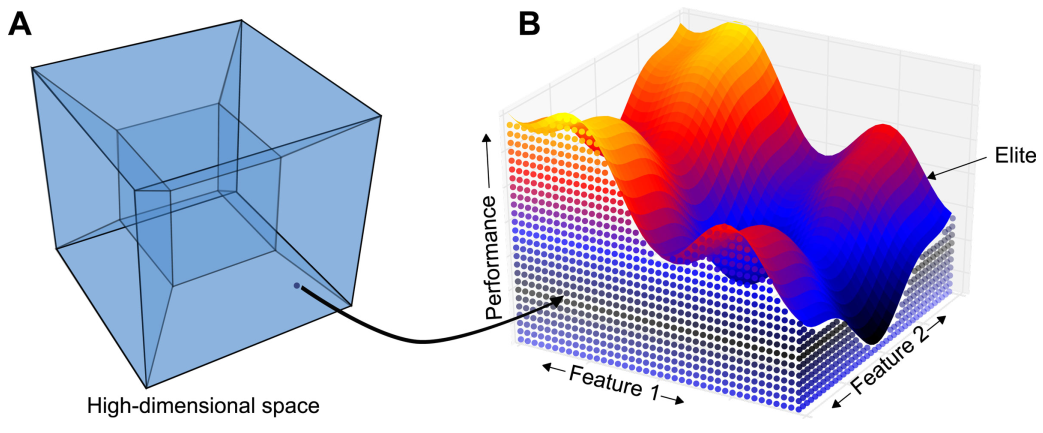
\includegraphics[width=0.7\textwidth]{Images/MAPElites.png}
    \caption{Visualization of the MAP-Elites algorithm.}
    \label{fig:mapelites}
\end{figure}

\textit{NS-LC} is also an illumination algorithm according to \citeauthor{mouret_illuminating_2015}, but they state that it is harder to understand and implement when compared to \textit{MAP-Elites}. They also show that \textit{MAP-Elites} performs empirically better than \textit{NS-LC}, by virtue of doing away with both the need to calculate the behavioral distance at each step, since it is implied in the archive itself, and with the need to maintain an archive of visited solutions separate from the current population, which NS-LS needs to avoid "cycling", the phenomenon where the population collectively moves back and forth between two regions of the behavior space. \cite{mouret_illuminating_2015}

\textit{MAP-Elites} has been used in a variety of domains and several variations have been developed in order to overcome certain limitations and adapt to specific needs. Some examples include \textit{Centroidal Voronoi Tessellations MAP-Elites} (CVT-ME) \cite{vassiliades_using_2017}, which scales the algorithm to high-dimensional spaces, \textit{Covariance Matrix Adaptation MAP-Elites} (CMA-ME) \cite{fontaine_covariance_2020} and \textit{Covariance Matrix Adaptation MAP-Annealing} \cite{fontaine_covariance_2022}, which doubles the performance of \textit{MAP-Elites} by combining the self-adaptation techniques of \textit{CMA-ES}\footnote{Covariance Matrix Adaptation Evolution Strategy is an advanced evolutionary optimization algorithm used for solving complex, non-linear, and multi-modal problems. It adapts the covariance matrix of the search distribution, allowing it to efficiently explore the search space by learning and exploiting the underlying structure of the problem.}, and \textit{Multi-Emitter MAP-Elites} \cite{cully_multi-emitter_2021}, which leverage a heterogeneous set of emitters to improve on \textit{Covariance Matrix Adaptation MAP-Elites}. Moreover, \textit{Constrained MAP-Elites} \cite{khalifa_talakat_2018}, \textit{MAP-Elites with Sliding Boundaries} (MESB) \cite{fontaine_mapping_2019} and other alternatives have been developed in the context of procedural content generation in games, which we will examine in the next section.

\subsection{Quality Diversity for procedural content generation in games}
\label{subsec:qd_pcg}
Among the many applications of QD methods across disciplines, such as optimization, robotics and machine learning, particularly relevant is their application to procedural content generation in games.

Quality Diversity is an appealing approach to PCG in games for a variety of reasons. 
While QD can generate a diverse set of high performing solution, constructive algorithms and machine learning methods produce instead a single artifact, search-based PCG is only concerned with the best-performing solution, and other declarative approaches, such as generative programming, while fast, lack the ability to control the diversity of the generated content. Moreover, QD considers more than one dimension of interest and leverages local competition instead of global competition, making it capable of exploring the fitness landscape better than other search-based methods. This allows QD to avoid deceptive fitness landscapes that may arise from the inherently difficult task of designing a fitness function. QD also generates, as a byproduct, the large set of artifacts needed to perform \textit{Expressivity Analysis}\footnote{The analysis of the output in terms of styles and variety of artifacts generated by the chosen approach, which can highlight biases of the generator towards specific types of content. \cite{gravina_procedural_2019}}, making it possible to run this process online during generation. Finally, QD is especially well-suited for mixed-initiative content design and offers \textit{explainability}\footnote{Explainable AI for Designers is an important research area that aims to aid the game designer in understanding AI algorithms applied to games. \cite{gravina_procedural_2019}} to the game designer thanks to its capability of showing a solution's lineage. \cite{gravina_procedural_2019} 


Notably, \textit{MAP-Elites} has been used to generate content for a variety of genres and some variations of the technique have been developed to fit specific needs. 

\citeauthor{khalifa_talakat_2018} have used \textit{MAP-Elites} to generate levels for bullet hell games. To that end, they developed a description language, \textit{Talakat}, capable of describing bullet hell levels, and a new technique called \textit{Constrained MAP-Elites}, which fuses the \textit{MAP-Elites} algorithm with the \textit{Feasible-Infeasible 2-Population} (FI2Pop) genetic algorithm\footnote{Genetic algorithm where two populations are kept, one of feasible and one of infeasible individuals. The feasible population is evolved to better its fitness, while the infeasible one to reduce their constraint violations, allowing the method to find more stepping stones. \cite{kimbrough_feasibleinfeasible_2008}} \cite{kimbrough_feasibleinfeasible_2008}. This new algorithm is able to evolve bullet hell levels described with \textit{Talakat} by keeping in each cell of the archive a population of feasible and infeasible levels, which are those levels that either satisfy a number of constraints or don't, and by evolving both populations simultaneously. Keeping two populations allows \textit{Constrained MAP-Elites} to find stepping stones between levels that would have otherwise been discarded immediately. Instead of defining a complex fitness function that describes "good" levels, a number of metrics are chosen as different dimensions of the \textit{Constrained MAP-Elites} and only playability is considered for the fitness function. \cite{khalifa_talakat_2018}

Several works have instead focused on platforming games. \Citeauthor{khalifa_intentional_2019} use \textit{Constrained MAP-Elites} to evolve a variety of playable \textit{Super Mario Bros.} levels which revolve around a specific game mechanic, using and comparing different simulation approaches to generate them \cite{khalifa_intentional_2019}. \Citeauthor{warriar_playmapper_2019} implemented \textit{PlayMapper}, a variation on the MAP-Elites algorithm, that is able to generate \textit{Super Mario Bros.} levels of different sizes and grants a significant amount of control over their generation, in contrast with popular black-box" AI techniques \cite{warriar_playmapper_2019}. \citeauthor{fontaine_illuminating_2021} apply some \textit{MAP-Elites} methods to illuminate the latent space of a \textit{Generative Adversarial Network (GAN)}\footnote{The latent space of a GAN is the space from which points are taken as input to generate new artifacts, and usually it's a vector. During training, the GAN learns how to map each point to generate an artifact.} trained on scenes from \textit{Super Mario Bros}. They focus on assessing the performance of QD algorithms on the task of generating scenes for \textit{Super Mario Bros.} with some specific characteristics \cite{fontaine_illuminating_2021}.

Another genre that has been the focus of QD research is that of "Zelda-like"\footnote{Games like The \textit{Legend of Zelda} (Nintendo EAD, 1986), where a player character traverses a world, fights enemies and beats dungeons made up of rooms with locked doors and keys.} adventure games, set in dungeons. 
\citeauthor{alvarez_empowering_2019} have used a new QD algorithm called \textit{Interactive Constrained MAP-Elites} to evolve dungeon rooms in \textit{Evolutionary Dungeon Designer} (EDD), a "mixed-initiative co-creativity"\footnote{The process of creating something by repeatedly having a human and a machine inspire each other through reciprocal stimuli.} tool. They leverage EDD's fitness and FI2Pop algorithm to develop an interactive version of \textit{Constrained MAP-Elites}, where the user guides the search towards satisfying results by choosing the features to explore and providing feedback on generated rooms \cite{alvarez_empowering_2019}. 
\citeauthor{charity_mech-elites_2020} searched for levels with specific mechanics in the \textit{GVG-AI Framework}'s games \cite{perez-liebana_general_2019}, which include a "Zelda-like" game \cite{charity_mech-elites_2020}. 
\Citeauthor{gonzalez-duque_finding_2020} used the \textit{Intelligent Trial-and-Error}\footnote{A form of Bayesian Optimization that uses MAP-Elites to generate the priors for a Gaussian Process} algorithm to perform \textit{Dynamic Difficulty Adjustment}, successfully producing levels of the desired difficulty for a "Zelda-like" game \cite{gonzalez-duque_finding_2020}. \citeauthor{viana_illuminating_2022} focused on generating entire levels, instead of single rooms, along with locked doors missions and enemy placement using MAP-Elites, while maintaining dungeon quality and providing a set of diverse levels \cite{viana_illuminating_2022}.

Some research has been done in the realm of puzzle games. \Citeauthor{charity_baba_2020} developed \textit{Baba is Y'all}, a mixed-initiative version of \textit{Baba is You}\footnote{Hempuli, 2019} where players design levels in collaboration with the machine. The game allows players to edit \textit{Baba is You} levels, similar to \textit{Super Mario Maker}\footnote{Nintendo EPD, 2015}, with the added goal of filling the archive of the underlying MAP-Elites algorithm, where levels are placed based on the combination of mechanics (rules) that are activated when solving them. The system can propose various starting levels for the user to edit based on what is already in the archive and what's currently missing to help players fill the archive \cite{charity_baba_2020}. 

MAP-Elites has also been used to generate powerful but diverse decks for \textit{Hearthstone}\footnote{Blizzard Entertainment, 2014}. \citeauthor{fontaine_mapping_2019} noted that \textit{MAP-Elites} uniformly divides the behavior space, however this can lead to a mismatch with the true distribution of the behavior space, which would result in a less effective illumination. Moreover, they argue that knowing \textit{a priori} this distribution can be hard or even impossible. To solve these issues, they propose \textit{MAP-Elites with Sliding Boundaries} (MESB), a variation of MAP-Elites where boundaries between cells are not placed uniformly based on the value of the features, but instead are dynamically placed at certain percentage marks of the distribution. A remap frequency is specified, meaning that the boundaries are periodically recalculated, allowing for a good estimation of the distribution of the search space. \cite{fontaine_mapping_2019}

Quality Diversity methods have yet to be applied to FPS games, be them singleplayer or multiplayer, which is where our research places itself.

\section{Summary}
\label{sec:ch1_summary}
In this chapter we have outlined the main concepts of level design in games, with a specific focus on competitive FPS games and academic research on them. We then explored the definition of "game balance", focusing on competitive games, and discussed the importance of map design in competitive FPS games to achieve balance. Furthermore, we have also discussed the main concepts of Procedural Content Generation in games, focusing on search-based methods and Evolutionary Algorithms in particular, and how they have been used to generate maps for FPS games. We have then introduced the concept of Quality Diversity and the MAP-Elites algorithm, explaining how they came to be and how they differ from traditional optimization methods. Finally, we have reviewed the main works that have used Quality Diversity methods to generate content for different genres of games, highlighting some relevant MAP-Elites variants such as MAP-Elites with Sliding Boundaries.
